\documentclass[12pt, a4paper, oneside]{article}\usepackage[]{graphicx}\usepackage[]{color}
%% maxwidth is the original width if it is less than linewidth
%% otherwise use linewidth (to make sure the graphics do not exceed the margin)
\makeatletter
\def\maxwidth{ %
  \ifdim\Gin@nat@width>\linewidth
    \linewidth
  \else
    \Gin@nat@width
  \fi
}
\makeatother

\definecolor{fgcolor}{rgb}{0.345, 0.345, 0.345}
\newcommand{\hlnum}[1]{\textcolor[rgb]{0.686,0.059,0.569}{#1}}%
\newcommand{\hlstr}[1]{\textcolor[rgb]{0.192,0.494,0.8}{#1}}%
\newcommand{\hlcom}[1]{\textcolor[rgb]{0.678,0.584,0.686}{\textit{#1}}}%
\newcommand{\hlopt}[1]{\textcolor[rgb]{0,0,0}{#1}}%
\newcommand{\hlstd}[1]{\textcolor[rgb]{0.345,0.345,0.345}{#1}}%
\newcommand{\hlkwa}[1]{\textcolor[rgb]{0.161,0.373,0.58}{\textbf{#1}}}%
\newcommand{\hlkwb}[1]{\textcolor[rgb]{0.69,0.353,0.396}{#1}}%
\newcommand{\hlkwc}[1]{\textcolor[rgb]{0.333,0.667,0.333}{#1}}%
\newcommand{\hlkwd}[1]{\textcolor[rgb]{0.737,0.353,0.396}{\textbf{#1}}}%

\usepackage{framed}
\makeatletter
\newenvironment{kframe}{%
 \def\at@end@of@kframe{}%
 \ifinner\ifhmode%
  \def\at@end@of@kframe{\end{minipage}}%
  \begin{minipage}{\columnwidth}%
 \fi\fi%
 \def\FrameCommand##1{\hskip\@totalleftmargin \hskip-\fboxsep
 \colorbox{shadecolor}{##1}\hskip-\fboxsep
     % There is no \\@totalrightmargin, so:
     \hskip-\linewidth \hskip-\@totalleftmargin \hskip\columnwidth}%
 \MakeFramed {\advance\hsize-\width
   \@totalleftmargin\z@ \linewidth\hsize
   \@setminipage}}%
 {\par\unskip\endMakeFramed%
 \at@end@of@kframe}
\makeatother

\definecolor{shadecolor}{rgb}{.97, .97, .97}
\definecolor{messagecolor}{rgb}{0, 0, 0}
\definecolor{warningcolor}{rgb}{1, 0, 1}
\definecolor{errorcolor}{rgb}{1, 0, 0}
\newenvironment{knitrout}{}{} % an empty environment to be redefined in TeX

\usepackage{alltt} % Paper size, default font size and one-sided paper
%\graphicspath{{./Figures/}} % Specifies the directory where pictures are stored
%\usepackage[dcucite]{harvard}
\usepackage{rotating}
\usepackage{amsmath}
\usepackage{setspace}
\usepackage{pdflscape}
\usepackage[flushleft]{threeparttable}
\usepackage{multirow}
\usepackage[comma, sort&compress]{natbib}% Use the natbib reference package - read up on this to edit the reference style; if you want text (e.g. Smith et al., 2012) for the in-text references (instead of numbers), remove 'numbers' 
\usepackage{graphicx}
%\bibliographystyle{plainnat}
\bibliographystyle{agsm}
\usepackage[colorlinks = true, citecolor = blue, linkcolor = blue]{hyperref}
%\hypersetup{urlcolor=blue, colorlinks=true} % Colors hyperlinks in blue - change to black if annoying
%\renewcommand[\harvardurl]{URL: \url}
\IfFileExists{upquote.sty}{\usepackage{upquote}}{}
\begin{document}
\title{Commodity Futures}
%\author{Rob Hayward\footnote{University of Brighton Business School, Lewes Road, Brighton, BN2 4AT; Telephone 01273 642586.  rh49@brighton.ac.uk}}
\date{\today}
\maketitle
\section*{Introduction}
Commodities are primarily traded in futures markets.  These are an agreement now to pay a particular price for a particular commodity at some set date in the future. These markets are mostly exchange traded and are therefore the quantities to be supplied and the dates at which this will be done are standardised.  Standardisation makes the contract more widely applicable and increases liquidity.  The difference between the underlying risk that is to be hedge by these contracts and the futures is called the \emph{basis risk}.  

The futures market is divided into two types of activity:  hedging and speculation.  The hedgers aim to reduce risk by locking in the price that they will buy or sell the commodity in the future.  For example, the oil hedgers will be oil companies, airline companies and other producers and users of oil and related products. The speculators taking a position in the market because they believe that they can make a profit from price movement. 

Keynes and Hicks argued that futures prices would tend to trade at a discount to the spot price because speculators would require some payment for taking risk from the hedgers. When the futures price is above the spot price or the price of the near future is above the far contract, this is called \emph{contango}; when the spot price is above the future or the near future is above the far future, this is called \emph{backwardation}

The US Commodity and Futures Trading Commission (CFTC), a regulatory body, requires that all participants in the futures market categorise themseleves as \emph{commerical} with some underlying business interest in the 

\section*{Pricing futures contracts}
The price of a futures contract should be equal to the cost of buying the commodity now and storing it until the delivery date.  For a financial serucity where the only cost is the cost of finance, the $F(t, T)$ futures price for time $T$, valued at $t$, where $t<T$ is equal to, 
\begin{equation*}
F(t, T) = S(t) \times (1 +r)^{(T-t)}
\end{equation*}
or, in continuous time, 
\begin{equation*}
F(t, T) = S(t)e^{r(T-t)}
\end{equation*}
For other futures, storage costs, income in the form of dividends and coupons and any other benefits that accrue from the holding of the commodity. This may be particularly important if there are large storage costs involved for commodities.

When there are disruptions in the supply of the commodity, this arbitrage mechanism will not work. In that case, the pricing will be determined by expections. 
\begin{equation*}
F(t, T) = E_t[S(T)]
\end{equation*}

The evolution of specultive positions shows that these positions have risen to near record levels.   
\begin{knitrout}
\definecolor{shadecolor}{rgb}{0.969, 0.969, 0.969}\color{fgcolor}

{\centering 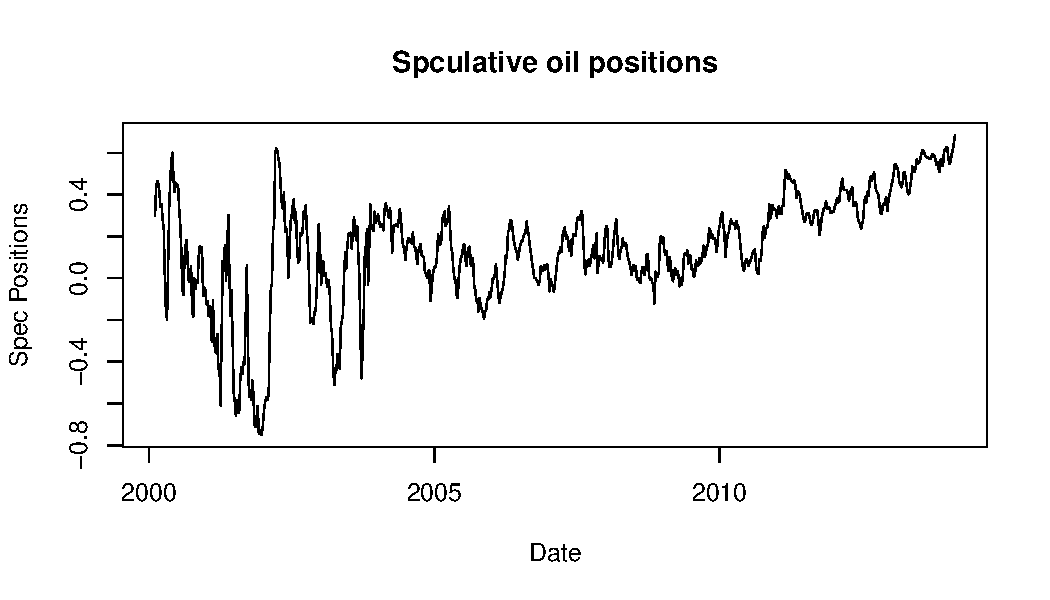
\includegraphics[width=\maxwidth]{figure/Oilspec} 

}



\end{knitrout}

However, the oil price remains below the highest levels. 

\begin{knitrout}
\definecolor{shadecolor}{rgb}{0.969, 0.969, 0.969}\color{fgcolor}
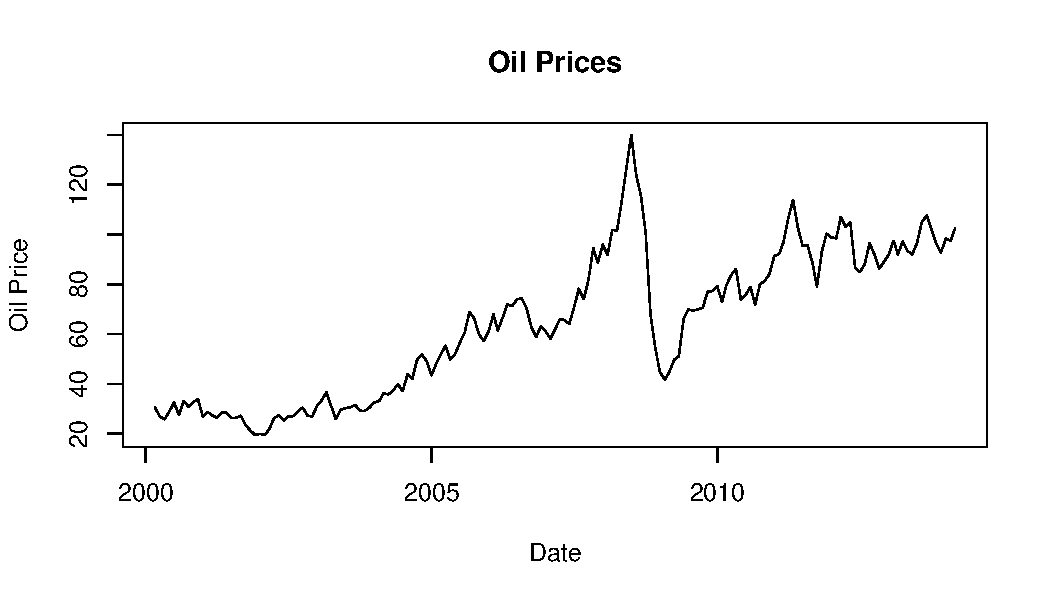
\includegraphics[width=\maxwidth]{figure/oilprice} 

\end{knitrout}


\section*{Delivery}
The futures contracts will expire in set months of March, June, September and December.  The actual time is determined by the exchange. The delivery is spefified by the contract.  For example, WTI is at the oil pipeline in Cushing Oaklahoma; Porkbellier are a particular quantity and quality of meat; bond futurs specify a particular range of bonds with particular coupons. 

\section*{Trading spreads}
There are two main benefits of using spreads:  

\begin{enumerate}
\item They can isolate a particular risk
\item They can reduce the total amount of risk
\end{enumerate}

Spreading can be a way of isolating particular risks or reducing the overall risk.  We have already looked at the spread between short-term interest rate (STIR) contracts that can be used to speculate on particular interest rate changes.  For example, the spread between December 2014 and December 2015 contract will be a play on interest rate expectation through the year 2015.  This can also be used to take a position on the performance of the economy.  Spreads are usually less risky.  For example, holding an outright short position for the December 2014 contract leaves you exposed to a sharp increase in the  value of the contract if there is any very positive economic news.  However, a short December 2014 position combined with  a long December 2015 position will reduce this risk as the increase in the price of December 2014 is likely to be mirrored to a great extent by an increase in the price of the December 2015 in many cases.  These are called \emph{calendar spreads}

Amongst the other spread trades are 
\begin{enumerate}
\item The \emph{Crack spread} is the spread between crude oil and oil products (gasoline and distillate fuel oil).  This is useful for oil refinary companies to manage the risk to their operations. The spread is linked to profitability. 
\item STIRS and bond futures will be a play on the yield curve.
\item STIRS in different currencies will play interest rate spreads. 
\item Bond futures will be spreads between bond markets. 
\item Gold vs Silver 
\item Oil vs gas
\end{enumerate}

The spead between the December 2014 and the December 2015 contracts will provide an indication of rate expectations for 2015.

The hedgers 
\begin{enumerate}
\item Oil companies hedging exposure to oil market
\item Airline companies hedging exposure to petroleum products.
\item Financial institutions hedging interst rate risk with STIRS, hedging bond issuance with the boind futures and funds covering exposure to stock market with equity futures. 
\end{enumerate}



Exchange rates are an exception.  For exchange rates, the spot market is more liquid than the futures. 




\end{document}
